\documentclass{subfiles}

\begin{document}
	\section{Previous Work}
	
	\par Regarding the integration of FW LiDAR and hyperspectral in remote forest surveys, there are diverse opinions on whether the integration of sensors improves remote forest surveying. Clark et al attempted to estimate forest biomass but no better results were observed after the integration \cite{Clark2011}, while the outcomes of Aderson et al for observing tree species abundances structures were improved after the integration of data \cite{Anderson2008}. 
	
	\par \cite{Buddenbaum2013} Buddenbaum et al, 2013, and \cite{Heinzel2012} Heinzel and Koch, 2012, used a combination of multi-sensor data for tree classifications. Buddenbaum et al use fusion of data to generate RGB images from a combination of FW LiDAR and hyperspectral features, although the fusion reduces the dimensionality of a classifier \cite{Buddenbaum2013}. Further, in their study, three different classifiers were implemented and the Support Vector Machines (SVMs) returns the best results. SVMs were also used in \cite{Heinzel2012} to handle the high dimensionality of the metrics (464 metrics). In that research a combination of FW LiDAR, discrete LiDAR, hyperspectral and colour infrared (CIR) images are used. Each of the 125 hyperspectral bands was directly used as a feature in the classifier, contributing to the high dimensionality. 
	
	\par Here some of the FW LiDAR and LiDAR features are used but in a digested form (i.e. the width of the waveform), and matches to the spectral signatures of each class are used to reduce the dimensionality.
	
	\par To enhance the visualisation of FW LiDAR data, a volumetric approach of polygonising the data was proposed by Miltiadou et al, 2014. First, the waveforms are inserted into a 3D discrete density volume, an implicit object is defined from the volume and the object is polygonised using the Marching Cubes algorithm. In this paper we emphasis the sampling of the volume versus the sampling of the Marching Cubes algorithm as well as the effects of using full-waveform versus discrete LiDAR. Further hyperspectral imagery is introduced to improve the visual output and allow parallel interpretation of the data.
	


	
\section{Integrating hyperspectral Imagery}


	\par For every scanned area, there are both FW LiDAR and hyperspectral data, but since the data are collected from different instruments they are not aligned. To integrate the data geo-spatially, aligning the data is required. In order to preserve the highest possible quality and reduce blurring that occurs during geo-rectification, data in original sense of geometry (level 1) are used. More Information about the hyperpsectral Imagery are available in Section \ref{sec:HyperspectralImages}.
	
	\par The main idea of the geo-recification is to find the nearest hyperspectral pixel to a point in the fastest possible way. For the reason, we first import the pixels into a 2D grid, similar to \cite{Warren2014}. The dimensions of the grid and the length of squares are constant, but in our case the average number of pixels per square $(A_{ps})$ can be modified and the dimensions $(n_x, n_y)$ of the grid are calculated as follow:
	
	\begin{eqnarray}
		n_x=\sqrt{\dfrac{n_s^2}{A_{ps}}} \;\;\;\;\;\;\;\;\;\; n_y=\sqrt{\dfrac{n_l^2}{A_{ps}}}   
	\end{eqnarray} 
	
	
	
%	\begin{math}
%	 $ \sqrt[root]{2} $
	 	
%	\end{math}
	
	\par where ns = the number of samples and
	nl = the number of lines in the hyperspectral images.
	
	\par Furthermore, while Warren et al use a tree-like structure, here  structure similar to hash tables is used to speed up searching. Hash table is a data structure, which maps keys to values. In our case, we utilise the unordered\_multimap available with the standard library of the $C++$ programming language, where for every key there is a bucket with multiple values stored inside. Each square $(x_s,y_s)$	has a unique key, which is equal to $(x_s + y_s *nXs)$ and each pixel is associated with the square it lies inside. In other words, every key with its bucket corresponds to a single square of the grid and every bucket includes all the pixels that lie inside that square. The next step is for every vertex $(x_v, y_v, z_v)$ to find the pixel whose geolocation is closest it. First we project each vertex into 2D by dropping the $z$ coordinate and then we find the square $(x_s , y_s )$ that its projection $(x_v , y_v)$ lies in, as follow:
	
	**** EQUATION *****
	
	**** EQUATION *****
	\par where maxX, minX, maxY, minY = the geolocation boundaries of all the hyperspectral image.
	
	\par From the square $(x_s,y_s)$ we can get the set of pixels that lie inside the same square with the vertex of our interest. Let’s assume that the positions and geolocations of these pixels are defined by $p_1	, p_2 , p_3, ... , p_n$ and $g_1, g_2, g_3 , ... , g_n$ respectively. Then, by looping through only that set of pixels, we can find the pixel $i$ that lies closest to the point $v(x_v , y_v)$
	
	**** EQUATION *****
	

	
	
		
\section{Visualisation}
	\par When the hyperspectral images are loaded along with the LiDAR files, then the outputs are: 	
	\begin{enumerate}
		\item the 3D geometry, which contains all the information about the vertices, edges, faces, normal and texture coordinates, and
		\item  a texture, which is an RGB image which is aligned with the texture coordinates of the polygon mesh.
	\end{enumerate}
	
	\par Here it worth mentioning that the texture coordinates $(u, v)$ of each vertex lies in the range $[0, 1]$ and if they are multiplied by the height/width of the texture, then the position of the corresponding pixel of the 2D texture is given. The 2D texture is simply an image generated from three user-selected bands for the RGB colours and its width is equal to the number of samples per line while its height is equal to the number of lines.
				
					
	\par DASOS projects level 1 hyperspectral images by adjusting the texture coordinates of the polygon according to the geolocation of the samples. That is, for each vertex $(xv, yv , zv)$ we find the pixel, whose geolocation $(x_g, y_g )$ is closest to it. Then by using the position of the pixel on the image $(x_p, y_p)$, the texture coordinates of the vertex are calculated accordingly.
				
	\par Finally, we need to scale the pixel position $p_i = (x_p, y_p )$, such that it lies in the range $[0,1]$. The scale factors are the number of samples $(n_s)$ and lines $(n_l)$ of the hyperspectral image. So, the texture coordinates $(u, v)$ of each vertex $v(x_v , y_v)$ are given by the following:
		
		
	**** EQUATION *****
	
	\subsection {Results}
		
		  \begin{figure} [h!]
		  	\centering
		  	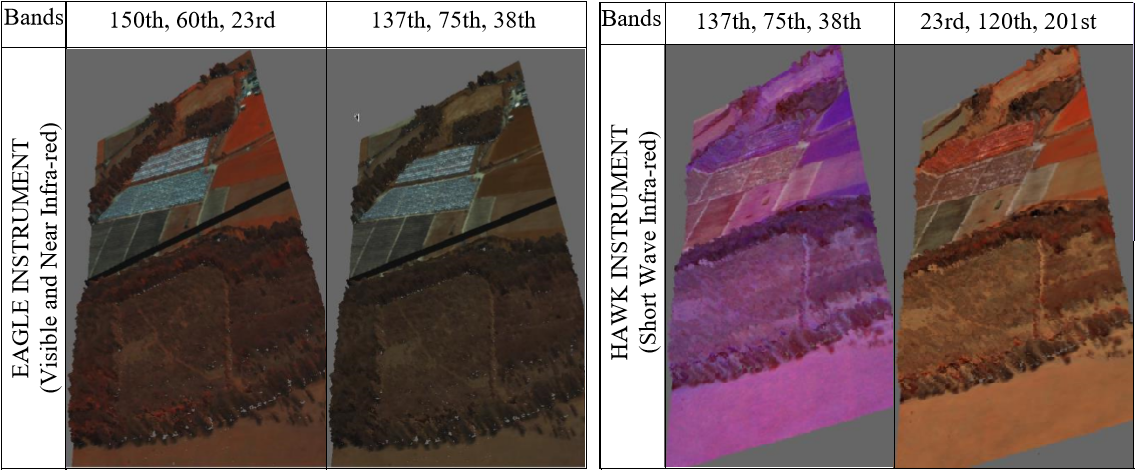
\includegraphics[width=\textwidth]{img/AlignmentEagle_Hawk}
		  	\caption[Results of Alignement]{Results of Alignment; the left table shows results of projecting hyperspectral images from the Eagle Instrument on polygonal meshes generated using FW LiDAR data and the right hand side images results using the Hawk instrument.}
		  	\label{fig:AlignementResults}
		  \end{figure}
		
		
\section{Tree Coverage Maps}

\par In Anderson et al, 2008, \cite{Anderson2008} an inverse distance weighted algorithm is used to raster the hyperspectral images and the pixel size is constant, 15.8m. While in this study an approach similar to Warren el \cite{Warren2014} is used and the resolution is changeable.

\par Further, the metrics generated from both hyperspectral and LiDAR are 2D aligned pictures. In other words, the pixel $(x, y)$ has the same geographical coordinates in every metric. Further the resolution of the metrics depends on the resolution of the 3D volume. If the dimensions of the volume are $(x, y, z)$ then the dimensions of the metrics are $(x, y)$. For LiDAR each pixel is coloured according to the information derived from the corresponding column. For Hyperspectral metrics level 1 data are used to preserve the highest possible quality. The same method as section 4.5 is used for finding the pixels from the hyperspectral data that are closest to the centre of the every column of the 3D discrete density volume.

\par The metrics used in this project are shown in the following table, but the list of the metrics can easily be extended. The metrics L1 to L4 are generated from the FW LiDAR data while the metrics H1 to H4 are generated from the hyperspectral images

\par To demonstrate the usefulness of DASOS, tree coverage maps are generated using a classifier and the results projected back into the polygon representations as shown in the following figure ***. A Naïve Bayesian classifier using a multi-variance Gaussian model is applied for distinguishing tree covered areas from the ground. The main idea is for each pixel/column to find the class
that is more likely to belong to (Tree or Ground).

\subsection{Results and Testing}
\par As expected the total accuracy was increased with the integration of FW LiDAR data and hyperspectral images. For validating the results, ground truth data were hand painted using 3D models generated with DASOS. Further there are three test cases and for each test case the following metrics are used:

1. L1-L4: Metrics generated from the FW LiDAR
2. H1-H4: Metrics generated from the hyperspectral
imagery
3. L1-L4 \& H1-H4: A combination of metrics generated from either FW LiDAR or hyperspectral imagery 

\par An error matrix represents the accuracy of the classifications (Congalton, 1991). Each row shows the number of pixels assigned to each class relative to their actual class. For example, the first row of Table 9 shows that 130445 pixels were classified as trees, where 125375 were actual trees and the rest 5070 were ground.

\par For each test case, an error matrix is generated to indicate the accuracy of the classification results as verified on the ground truth data (Table 9-11). From the error matrices the classification accuracy of each test case was calculated and is
presented in the Table 12.


** Tables ***

\par Figure 13 depicts the coverage maps generated for each test case. Three areas were also marked for comparison. Area 1 has been wrongly classified when only the hyperspectral data were used; nevertheless with the height information of the LiDAR
data, area 1 was correctly classified. Similarly, area 2 was wrongly classified using the FW LiDAR because the height of the trees were less than the training samples but since the hyperspectral images do not contain height information, the
trees were better labelled at the related test cases. By the end area 3 contains greenhouses, which seems to confuse the first two classifications in different ways, while the combination is much improved. 


*** Image *** 

\section {Summary and Conclusions}
\par In this paper we showed an efficient way of aligning the FW LiDAR data and hyperspectral images. The voxel representation of the FW LiDAR data eases the handling of data as well as the alignment with the hyperspectral images. Furthermore, the spatial representation of hyperspectral pixels into a grid
contributes to the efficiency of the alignement.

\par The visualisation of FW LiDAR data and hyperspectral images has been improved by introducing computer graphics approaches to remote sensing. While the state-of-the-art FW LiDAR visualisations talks about points clouds and transparent
voxels, the output of DASOS is a coloured polygon representation which can be exported and interpretated in modeling softwares, like Meshlab.

\par It was also showed that the integration of the data has great potentials in remote forest surveys. This was demonstrated using a Bayesian probabilistic classifier for generating tree coverage maps. Positive results were shown by improved classification accuracy when both datasets were used.

\par By the end, the tools developed for this research are now openly available (Section 2). 

\end{document}